% Tento soubor nahraďte vlastním souborem s obsahem práce.
%=========================================================================
% Autoři: Michal Bidlo, Bohuslav Křena, Jaroslav Dytrych, Petr Veigend a Adam Herout 2019
\chapter{Úvod}
\label{chapter:uvod}
Nejprve je nutné poznamenat, že zadání práce bylo velice obecné. Na zadání \enquote{Simulace kapalin na GPU} může být aplikováno mnoho řešení, a to nejen v~rámci modelovaného fenoménu, ale i použitých technologií a metod. Lze například simulovat jednoduchou scénu padajícího objemu dané kapaliny. Další možností je například simulace interakce mezi dvěma druhy kapalin. Bylo by i možné vytvořit systém eroze, kdy by kapalina deformovala a ničila podloží a obecně pevná tělesa představená do systému. Další možností je simulace fyzikálních vlastností kapalin. Zároveň je dostupných mnoho metod jak k~simulaci přistoupit. Lze využít mřížkové metody počítající hodnoty v~předem definovaných místech, či redukovat paměťovou náročnost a využít řídkých mřížek. Možností je i využití celulárních automatů pro velmi jednoduché simulace, či využít například částicového přístupu pro mnohem složitější a fyzikálně přesnější simulace.

Tato práce se nejvíce zaměřovala na modelování fyzikálních vlastností kapalin. Přesněji řečeno se jedná o~simulaci kondenzace a vypařování. V~celém systému by měly být jasně odlišitelné jednotlivé fáze a kapalina by v~závislosti na teplotě měla plynule přecházet mezi skupenstvím kapalným a plynným. V~systému by tedy měla být jasná hladina s~kapalinou, její výpary a zkondenzované kapičky. Co se týče použitých metod, jsou v~práci zastoupeny dva hlavní přístupy pro modelování toku kapalin či plynů. Pro simulaci kapaliny je využito částicového přístupu, přesněji metody Smoothed Particle Hydrodynamics představené autory Monaghan \cite{Monaghan77} a Lucy \cite{Lucy77}. Pro simulaci plynného skupenství je pak využito mřížkové metody představené v~roce 1999 autorem Jos Stamem. \cite{Stam99} Aby docházelo ke správnému přenosu informací mezi jednotlivými systémy, je nutné propojit obě metody mezi sebou, a zároveň je propojit s~pevnými tělesy.

Využití takového systému by pak mohlo být například při demonstraci daného jevu studentům a ukázání chování kapaliny v~různých situacích. Nicméně hlavním cílem této práce je nejen vytvořit daný systém, ale hlavně prozkoumat možnosti simulace kapalin. Primárním cílem tedy bylo prozkoumat různé metody modelování kapalin a tyto poznatky následně uplatnit při tvorbě samotné aplikace, čehož bylo docíleno především zvolením článku \cite{Evap&Cond} autorů Hendrika Hochstettera a Andrease Kolba z~University of Siegen v~Německu, zabývajícího se zmíněnou kondenzací a vypařováním a využívající dvě různé metody simulace.


\chapter{Teorie}
Následující kapitola se věnuje vysvětlení základní teorie skrývající se za simulacemi a animacemi tekutin a plynů. Nejprve je zde obecně vysvětlen pojem simulace a animace kapalin. Dále jsou zde vysvětleny různé přístupy k~simulaci, je zde vysvětlena mřížková neboli Lagrangeova metoda a částicový přístup neboli Eulerova metoda. V~každé sekci jsou následně popsány některé významné algoritmy spadající pod jednotlivé metody.

\label{chapter:teorie}
\section{Simulace kapalin}
Nejprve je nutné odlišit pojmy simulace kapalin a animace kapalin. V~obou případech jde především o~chování kapaliny v~určité situaci, nicméně animace se oproti simulaci zaměřuje především na vizuální stránku a méně na fyzikální přesnost. Jedná se tedy pouze o~aproximaci vzorců popisujících chování kapalin například zanedbáním velké části objemu kapaliny a popisem pouze chování hladiny kapaliny (viz níže). Jedním z~možných využití takových aproximací jsou případy, kde natolik nezáleží na přesnosti chování, jako spíše na vizuální stránce. Příkladem mohou být videohry, ve kterých je nutné mít vizuálně přívětivou kapalinu, ale zároveň vypočitatelnou v~reálném čase s~přihlédnutím na výpočet mnoha dalších jevů v~rámci herního enginu. Avšak například při tvorbě animací a vizuálních efektů pro filmy, kde nejsme omezeni časem, lze využívat mnohem výpočetně náročnějších animací. Tyto animace sice stále nemusí být fyzikálně dokonalé, jedná se však o~mnohem propracovanější vyobrazení kapalin, než pouhé vlnění hladiny. \cite{Medvecky-Heretik2018thesis}

\begin{figure*}[h]\centering
	\centering
	\captionsetup{justification=centering}
	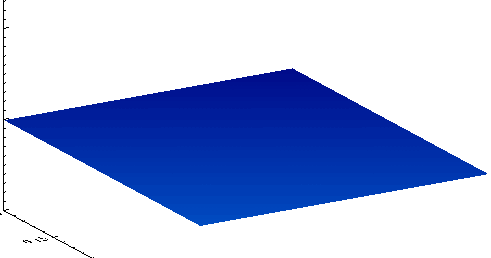
\includegraphics[width=0.3\linewidth]{obrazky-figures/SurfaceWaves/SurfWave_01.png}\hfill
	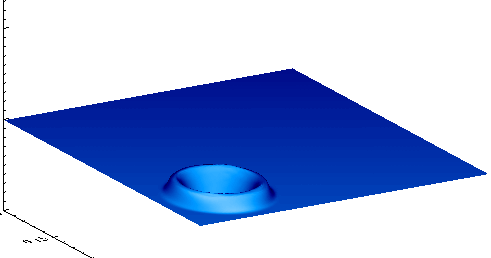
\includegraphics[width=0.3\linewidth]{obrazky-figures/SurfaceWaves/SurfWave_02.png}\hfill
	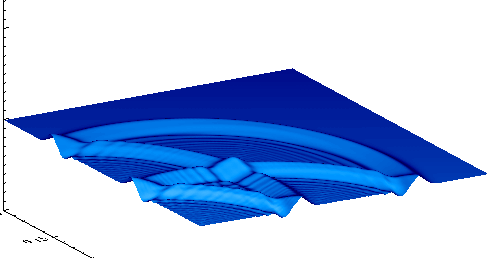
\includegraphics[width=0.3\linewidth]{obrazky-figures/SurfaceWaves/SurfWave_03.png}\hfill
	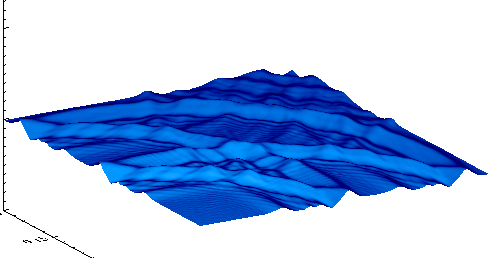
\includegraphics[width=0.3\linewidth]{obrazky-figures/SurfaceWaves/SurfWave_04.png}\hfill
	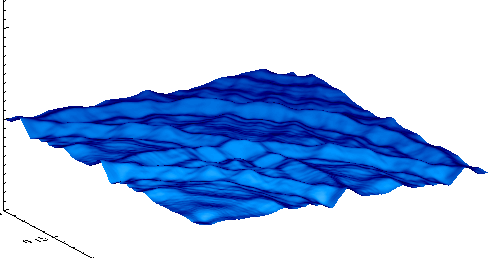
\includegraphics[width=0.3\linewidth]{obrazky-figures/SurfaceWaves/SurfWave_05.png}\hfill
	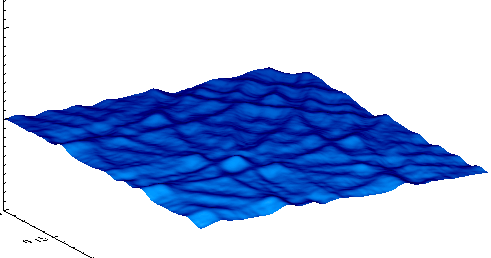
\includegraphics[width=0.3\linewidth]{obrazky-figures/SurfaceWaves/SurfWave_06.png}\hfill
	\caption{\textbf{Shallow Water Equation.} Postupné šíření vln při několika kapkách vody.}
	\textbf{Zdroj: } \url{https://en.wikipedia.org/wiki/Shallow_water_equations}
	\label{fig:SWE}
\end{figure*}

\subsubsection{Simulace hladiny}
Simulace vlnění hladiny je jedna z~nejjednodušších vizualizací kapaliny. Existuje samozřejmě více přístupů jak takovou simulaci realizovat, mezi které patří například výškové mapy, vlnová funkce či rovnice mělké vody (Shallow Water Equation). Ačkoliv produkují v~celku uspokojivé vlnění hladiny, existují v~okolním světě běžné jevy, jako například lámající se vlny, které za pomocí jednoduchých vlnových funkcí a výškových map nelze simulovat. \cite{Medvecky-Heretik2018thesis}

\begin{figure}[hbt]
	\centering
	\captionsetup{justification=centering}
	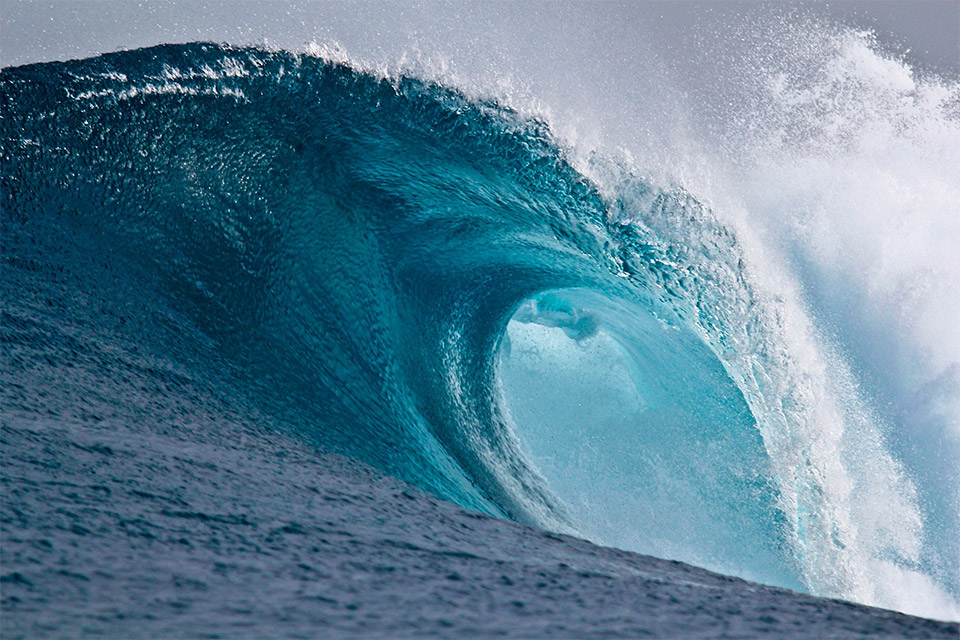
\includegraphics[width=0.4\textwidth]{obrazky-figures/Large_breaking_wave.jpg}
	\caption{\textbf{Lámající se vlna.} Jev v~reálném světě, který není realizovatelný za pomocí výškových map a vlnových funkcí.}
	\textbf{Zdroj: } \url{https://en.wikipedia.org/wiki/Breaking_wave}
	\label{keepCalm}
\end{figure}

Simulace kapalin se naopak snaží být oproti animacím co nejvíce fyzikálně přesné, čímž ale rapidně vzrůstá náročnost výpočtů. Existuje nespočet metod jak dosáhnout výsledku, nicméně čím přesnější a složitější scéna, tím delší výpočet daného scénáře. Doba výpočtu se tak může pohybovat v~rámci minut, ale i hodin. Tyto metody jsou pak často založeny nad numerickými výpočty fyzikálních rovnic, kde nejpoužívanější rovnice jsou rovnice Navier-Stokes.

\subsection{Navier-Stokesovy rovnice}
Navier-Stokesovy rovnice jsou jedny z~nejvyužívanějších rovnic pro výpočty chování kapalin. Základy pro popis dynamiky kapalin položil již v~roce 1687 Sir Isaac Newton v~článku "Principa", kde bylo poprvé správně popsáno chování viskózních kapalin. Později Daniel Bernoulli a Leonhard Euler popsali chování neviskózního toku pomocí rovnic dnes známých jako Eulerovy neviskózní rovnice (Euler’s inviscid equations). Až Claude-Louis Navier a Sir George Stokes na sobě nezávisle odvodili finální podobu rovnic ze zmiňovaných Eulerových a Newtonových rovnic. Tyto Navier-Stokesovy rovnice jsou nyní nejpoužívanější formou popisu chování kapalin a bylo na nich postaveno nespočet různých algoritmů. \cite{simscale_2020}

\begin{equation}
	\rho(\frac{\partial}{\partial t} + \mathbf{u} \cdot \nabla)\mathbf{u} = -\nabla p + \mu\nabla\cdot(\nabla \mathbf{u}) + f
	\label{eq:NavierStokes}
\end{equation}

\begin{equation}
	\nabla \cdot \mathbf{u} = 0
	\label{eq:NavierStokes2}
\end{equation}

Tři základní vlastnosti viskózní kapaliny, která má neměnné teplo, jsou rychlost ($\mathbf{u}$), tlak ($p$) a hustota ($\rho$). V~rovnici \ref{eq:NavierStokes} pak $\mu$ označuje viskozitu kapaliny a $f$ ostatní síly působící na kapalinu, jako například gravitace. Tyto rovnice tudíž vyjadřují zákon o~zachování hybnosti a zákon o~zachování hmotnosti pro Newtonské kapaliny. Newtonská kapalina je pak kapalina kterou lze popsat lineárním Newtonovým modelem. Její viskozita je pak závislá především na tlaku a teplotě a z~tohoto hlediska se jedná o~takzvanou Newtonskou viskozitu. U~nenewtonské kapaliny pak popisujeme takzvanou zdánlivou viskozitu závislou na předchozí deformaci kapaliny a rychlosti vnitřního smyku kapaliny. Tyto kapaliny pak nelze popsat lineárním Newtonovým zákonem.\cite{StejskalJan2013Pmks}

Navier-Stokesovy rovnice jsou hojně využívány nejen pro simulaci a animaci kapalin, ale v~celé řadě dalších vědních oborů. Využití můžeme nalézt při vytváření modelů pro předpověď počasí, pro studování toku vzduchu při výrobě letadel nebo například při analýze šíření znečištění.
\break

Existují dva úhly pohledu na organizaci a řešení nejen těchto rovnic, ale zároveň obecně na řešení dynamiky kapalin. Tyto metody se pak liší především v~bodech pozorování. V~Eulerově metodě dochází k~výpočtu požadovaných hodnot v~přesně daných bodech, tedy v~určité diskrétní mřížce. U~Lagrangeovy metody dochází k~výpočtu v~bodech sledované masy, tedy v~částicích sledované kapaliny. Dále jsou obě metody detailněji popsány, včetně několika algoritmů, které pod dané metody spadají.

\begin{figure}[h]
	\centering
	\begin{subfigure}{.5\textwidth}
		\centering
		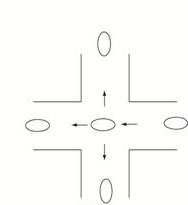
\includegraphics[width=0.7\linewidth]{obrazky-figures/EulerLagran_02.jpg}
		\caption{\textbf{Eulerův přístup}}
		\label{fig:Euler}
	\end{subfigure}%
	\begin{subfigure}{.5\textwidth}
		\centering
		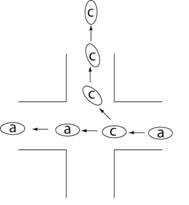
\includegraphics[width=0.7\linewidth]{obrazky-figures/EulerLagran_01.jpg}
		\caption{\textbf{Lagrangeův přístup}}
		\label{fig:Lagran}
	\end{subfigure}
	\caption{\textbf{Příklad dvou přístupů nad křižovatkou s~auty.} Eulerův přístup (\ref{fig:Euler}) sleduje křižovatku v~předem daných místech (ramena a střed křižovatky). Naopak Lagrangeův přístup(\ref{fig:Lagran}) sleduje konkrétní vozidla (a,c), jak projíždí křižovatkou.}
	\textbf{Zdroj:} \url{http://abe-research.illinois.edu/faculty/dickc/Engineering/ELdescrip2a.htm}
	\label{fig:ztencovani}
\end{figure}

\section{Eulerova metoda toku}
Jak bylo popsáno výše, při využití Eulerovy metody jsou vlastnosti kapaliny počítány v~pevně definovaných bodech diskrétní mřížky. Ačkoliv některé vlastnosti kapaliny popisuje Eulerova metoda mnohem přesněji, největší nevýhodou je samotná mřížka. Jeden z~prvních problémů je hrubost mřížky. Podíváme-li se na Obr.\ref{fig:EulerGrid} je patrné, že reálná hladina je lehce zvlněná, ale z~důvodu velké hrubosti mřížky a tedy hrubějšímu vzorkování, by lehké zvlnění bylo zanedbáno a hladina by byla rovná.

Dalším problémem je paměťová náročnost. Snažíme-li se vytvořit jemnější mřížku, abychom odstranili problémy související s~hrubou mřížkou, musíme počítat se zvyšující se paměťovou náročností. Pokud se pohybujeme ve trojrozměrném prostoru a chceme-li zpřesnit v~každé ose mřížku dvakrát, musíme počítat s~osminásobně více buňkami v~paměti. Tento problém však naštěstí lze již řešit pomocí různých struktur jako jsou například řídké mřížky.
\todo{popis řídké mřížky}

Posledním problémem je samotná uzavřenost mřížky, která brání k~plně dynamické simulaci. Kapalina je tedy uzavřena do \enquote{nerozbitné nádoby} a jakýkoliv pokus o~její tok mimo mřížku je nemožný. I~na tento problém však existuje řešení, a to v~podobě dynamických mřížek, které se v~případě nutnosti dokáží rozšiřovat v~prostoru a poskytnout tak prostor pro rozsáhlejší simulační prostor.
\cite{KelagerSPH}

\begin{figure}[hbt]
	\centering
	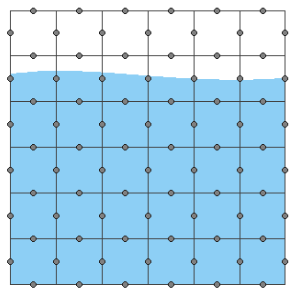
\includegraphics[width=0.4\textwidth]{obrazky-figures/GridEuler.PNG}
	\caption{\textbf{Eulerova mřížka.} Kapalina uzavřená ve 2D mřížce. Rychlost kapaliny je reprezentována ve vyznačených tečkách.}
	\textbf{Zdroj: } Lagrangian Fluid Dynamics Using Smoothed Particle Hydrodynamics \cite{KelagerSPH}
	\label{fig:EulerGrid}
\end{figure}

\subsection{Mřížková metoda}
\label{chapter:Grid}
Mřížková (Grid) metoda je Eulerovská metoda využívající pro pohyb kapaliny několika polí vektorů. Základem mřížkové metody je pole vektorů rychlostí pro každý zkoumaný bod v~mřížce. Toto pole pak představuje pohyb tekutiny v~celém zkoumaném prostoru.
\begin{equation}
	\Vec{u}(x,y) = (u_x,u_y)
\end{equation}

\begin{figure}[hbt]
	\centering
	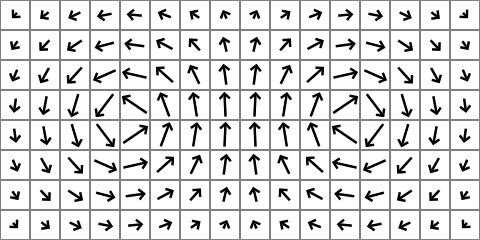
\includegraphics[width=0.5\textwidth]{obrazky-figures/flow-field.png}
	\caption{\textbf{Pole rychlostí.} Šipky v~poli označují velikost a směr proudění.}
	\textbf{Zdroj: } \url{https://www.karlsims.com/fluid-flow.html}
	\label{fig:EulerGrid}
\end{figure}

Dalším základním stavebním kamenem algoritmu je pak advekce, neboli přesun vlastností z~jednoho místa na jiné v~důsledku pohybu kapaliny. Uvažujeme-li, že tok kapaliny přenáší například určitou koncentraci částic (kouř, barvivo, písek), pak máme dvě možnosti jak posunout dané hodnoty v~čase a prostoru.  První možností je dopředný posun v~čase. V~závislosti na pozici $\mathbf{r}$ zvolíme odpovídající rychlost $\mathbf{u}$ a danou hodnotu $A$ posuneme v~prostoru.

\begin{equation}
	A(\mathbf{r} + \mathbf{u}\Delta t, t + \Delta t) = A(\mathbf{r}, t)
\end{equation}

Druhým možným přístupem pro přesun hodnot je tzv. backtracking. V~tomto přístupu není hodnota posunuta z~jedné pozice na druhou. Nicméně se vektor rychlosti invertuje a do nynější pozice se přesouvá pozice předchozí. \cite{webglFluid}

\begin{equation}
	A(\mathbf{r}, t + \Delta t) = A(\mathbf{r} - \mathbf{u}\Delta t, t)
\end{equation}

Stejně jako přesouváme určité částice v~prostoru, můžeme přesouvat i pole rychlostí a měnit jej tak v~čase. V~tomto případě však můžou nastat problémy s~nestlačitelností a zákonem zachování hmotnosti. Musíme tedy zaručit, že divergence pole rychlosti je všude nulová. Divergence nám zjednodušeně říká, zda v~určitém bodě daná vlastnost roste, či klesá. Chceme-li tedy docílit nulové divergence pole rychlosti, chceme vlastně docílit toho, že nám v~žádném bodě neklesá ani neroste hustota kapaliny. \cite{webglFluid}

\begin{figure}[h]
	\centering
	\begin{subfigure}{.3\textwidth}
		\centering
		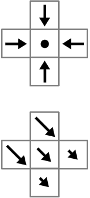
\includegraphics[width=0.35\linewidth]{obrazky-figures/div-negative.png}
		\caption{\textbf{Záporná divergence}}
		\label{fig:Euler}
	\end{subfigure}%
	\begin{subfigure}{.3\textwidth}
		\centering
		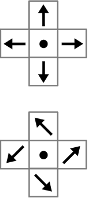
\includegraphics[width=0.35\linewidth]{obrazky-figures/div-positive.png}
		\caption{\textbf{Kladná divergence}}
		\label{fig:Lagran}
	\end{subfigure}
	\begin{subfigure}{.3\textwidth}
		\centering
		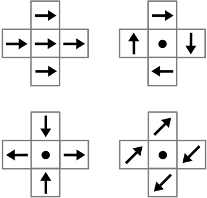
\includegraphics[width=0.8\linewidth]{obrazky-figures/div-zero.png}
		\caption{\textbf{Nulová divergence}}
		\label{fig:Lagran}
	\end{subfigure}
	\caption{Příklady různých divergencí v~bodě, v~závislosti na velikosti a směru vektorového pole v~okolí.}
	\textbf{Zdroj:} \url{https://www.karlsims.com/fluid-flow.html}
	\label{fig:div}
\end{figure}

Při výpočtu pole s~nulovou divergencí nám pomůže takzvaný Helmholtz-Hodgeův rozkladový teorém.

\begin{equation}
	\mathbf{u} = \mathbf{w} - \nabla p
	\label{eq:HelmHodge}
\end{equation}

Kde $\mathbf{u}$ je naše hledané pole s~nulovou divergencí, $\mathbf{w}$ je pole rychlostí s~nenulovou divergencí a $\nabla p$ je gradient tlaku. Tato rovnice nám tedy říká, že pole rychlostí s~nenulovou divergencí může být opraveno pomocí gradientu tlaku. Pro výpočet tlaku lze pak odvodit ze stejného teorému \ref{eq:HelmHodge} následující rovnici. \cite{webglFluid}

\begin{equation}
	p_{x,y}^{(k+1)} = \frac{p_{x+1,y}^{(k)} + p_{x-1,y}^{(k)} + p_{x,y+1}^{(k)} + p_{x,y-1}^{(k)} + \alpha b_{x,y}}{\beta}
\end{equation}

Kde pro neviskózní kapaliny platí, že $\alpha = -( velikost\_bunky )^2$, $\beta = 4$ a $b = \nabla \cdot \mathbf{w}$. Tato rovnice je pak řešena Jacobiho iterativní metodou, kde počáteční odhad je nulový tlak ve všech bodech. Po dostatečném počtu iterací dostaneme hodnotu tlaku ve všech bodech a po výpočtu gradientu a aplikování ve vzorci \ref{eq:HelmHodge} získáme pole rychlostí s~nulovou divergencí. Pomocí tohoto pole pak lze posouvat výše zmíněné hodnoty jako je barva, koncentrace částic a jiné.
\cite{GPUGemsGridFLuid}

\begin{figure}[hbt]
	\centering
	\captionsetup{justification=centering}
	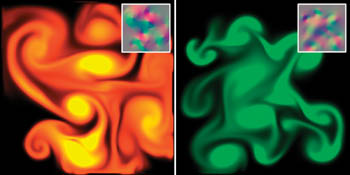
\includegraphics[width=0.5\textwidth]{obrazky-figures/GridFluid.jpg}
	\caption{\textbf{Mřížková metoda.} Vizualizace barviva v~proudící vodě.}
	\textbf{Zdroj: } Chapter 38. Fast Fluid Dynamics Simulation on the GPU \cite{GPUGemsGridFLuid}
	\label{fig:EulerFluid}
\end{figure}

\todo{využití, výhody/nevýhody}
\subsection{Celulární automaty}
Pro simulaci toku kapalin lze využít i celulárních automatů. Celulární automat se skládá z~několika důležitých částí, stavového prostoru rozděleného na diskrétní buňky, přechodové funkce a množiny stavů, které mohou buňky nabývat. Celulární automaty pracují na principu $n$-dimenzionálního okolí, kde $n$ závisí na dimenzi zkoumaného prostoru a typu okolí. V~jednom časovém kroku se pak aplikuje na všechny buňky přechodová funkce, která vyhodnotí stavy okolních buněk a podle výsledku nastaví vlastní stav.

\begin{figure}[hbt]
	\centering
	\captionsetup{justification=centering}
	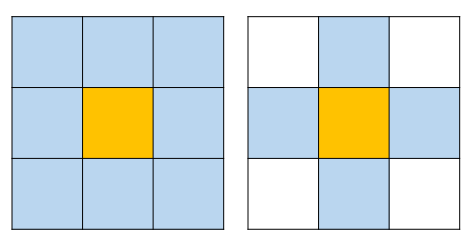
\includegraphics[width=0.5\textwidth]{obrazky-figures/Neighborhood.png}
	\caption{\textbf{Typy okolí.} Vlevo Moorovo okolí, vpravo Von-Neumanovo}
	\textbf{Zdroj: } \url{http://complextin.blogspot.com/2016/06/2d-cellular-automata-three-state.html}
	\label{fig:EulerFluid}
\end{figure}

Pomocí popsaného principu a využití několika jednoduchých pravidel pak lze vytvořit velice jednoduchý simulátor toku vody. Nejdříve se simuluje působení gravitace a automat se pokusí co nejvíce vody přesunout o~buňku níže. Pokud je buňka plná nebo se jedná o~buňku, do které nemůže téci voda, zbylá kapalina je distribuována do okolních horizontálních buněk. Jedná se o~velice jednoduchý algoritmus, který však zanedbává mnoho vlastností kapalin. Prvním problémem je situace při spojených nádobách, kdy pomocí tohoto algoritmu nedojde k~vyrovnání hladin a je nutné aplikovat další procesy pro vyrovnávání hladin. Dalším problémem je odrazivost a rychlost toku kapalin. Kapalina se bude vždy pohybovat stejnou rychlostí a představíme-li si situaci kdy \enquote{naráží} do stěny, pak nedojde k~roztříštění a případnému stoupání kapaliny vzhůru. Dalším problémem mohou být vlastnosti kapaliny, jako je například viskozita, která se zanedbává, případně může být simulována pouhým koeficientem ovlivňujícím rychlost toku. \cite{Medvecky-Heretik2018thesis}
\todo{využití, obrázky}

\begin{figure*}[h]\centering
	\centering
	\captionsetup{justification=centering}
	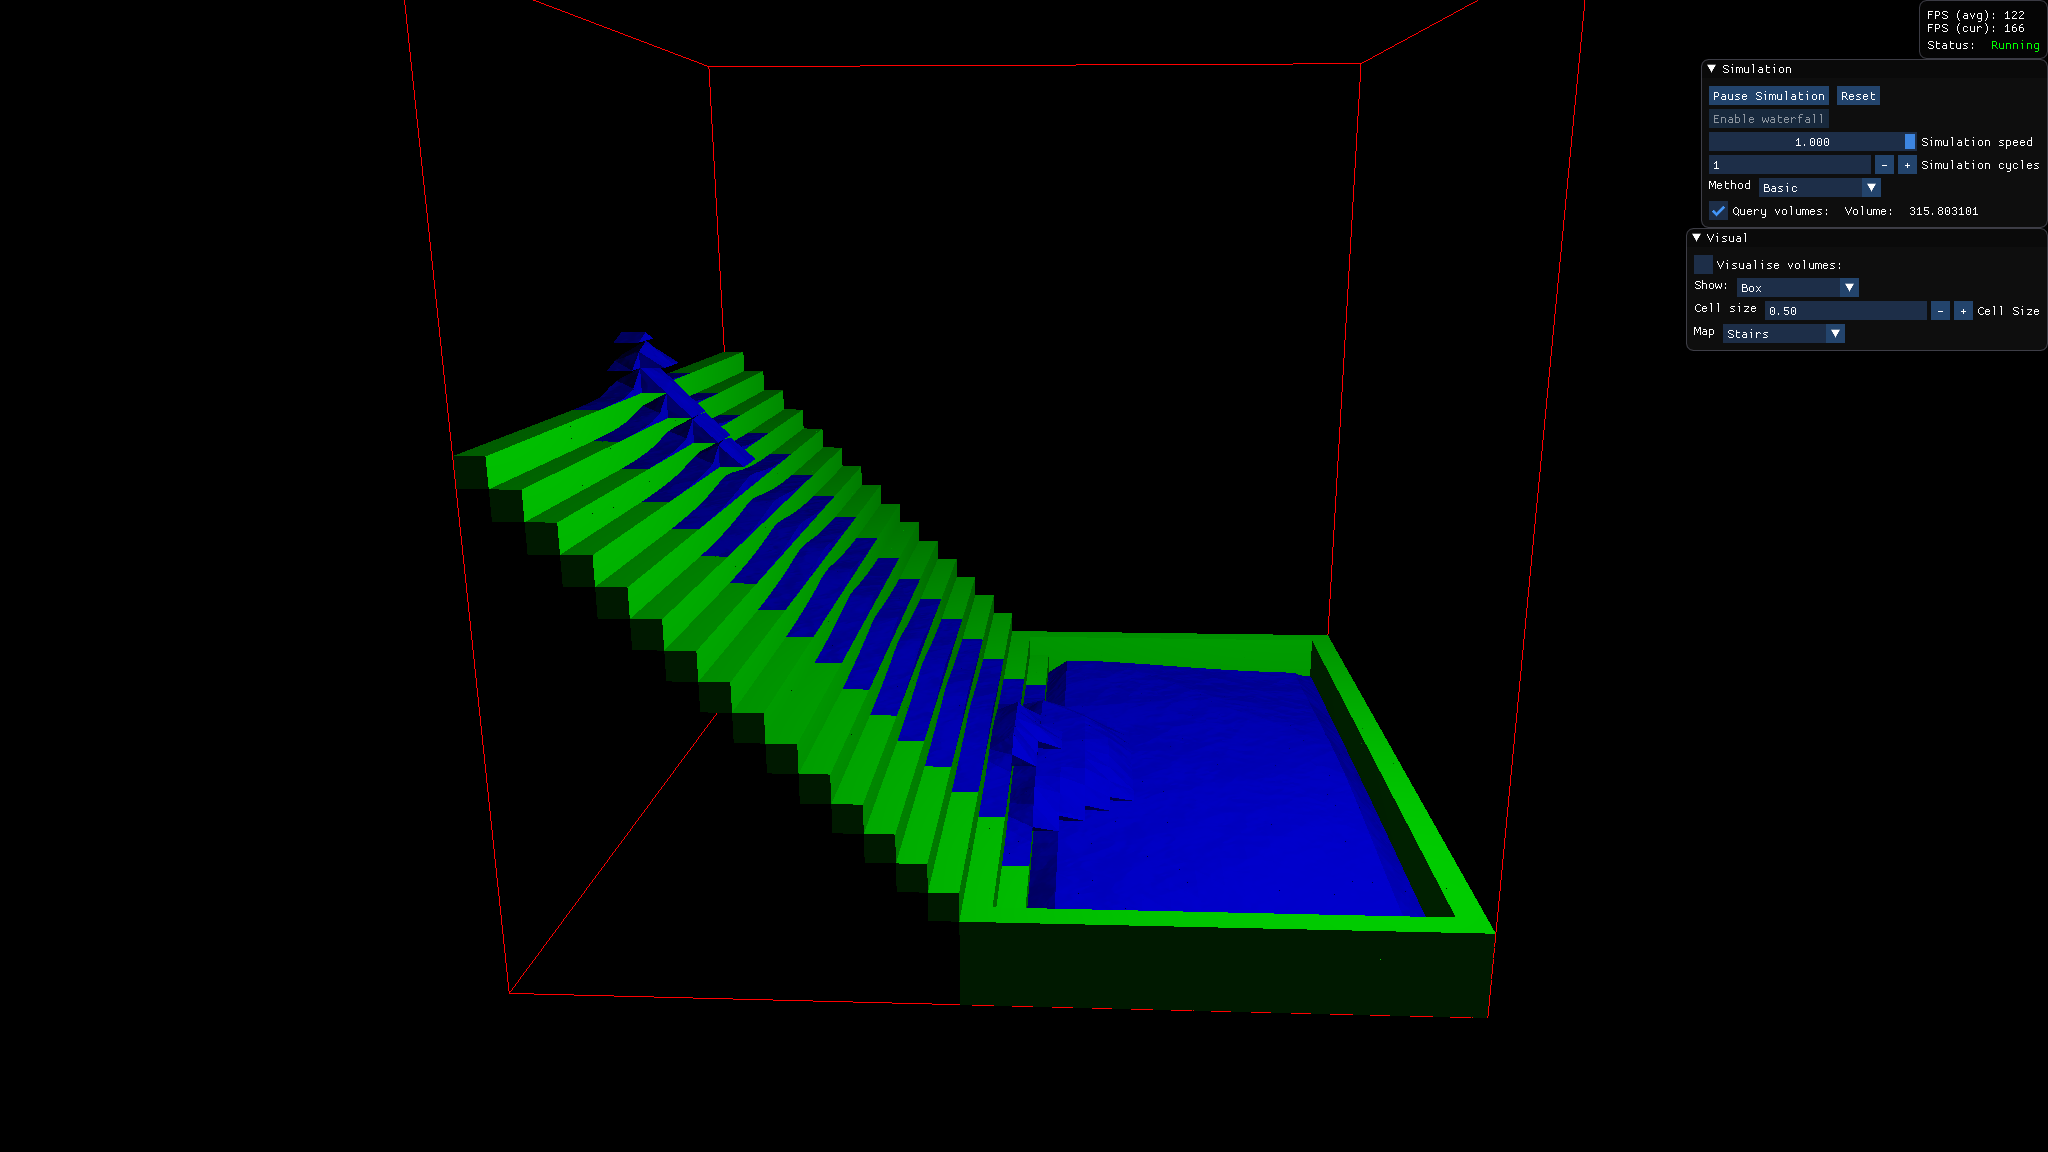
\includegraphics[width=0.5\linewidth]{obrazky-figures/cellular1.png}\hfill
	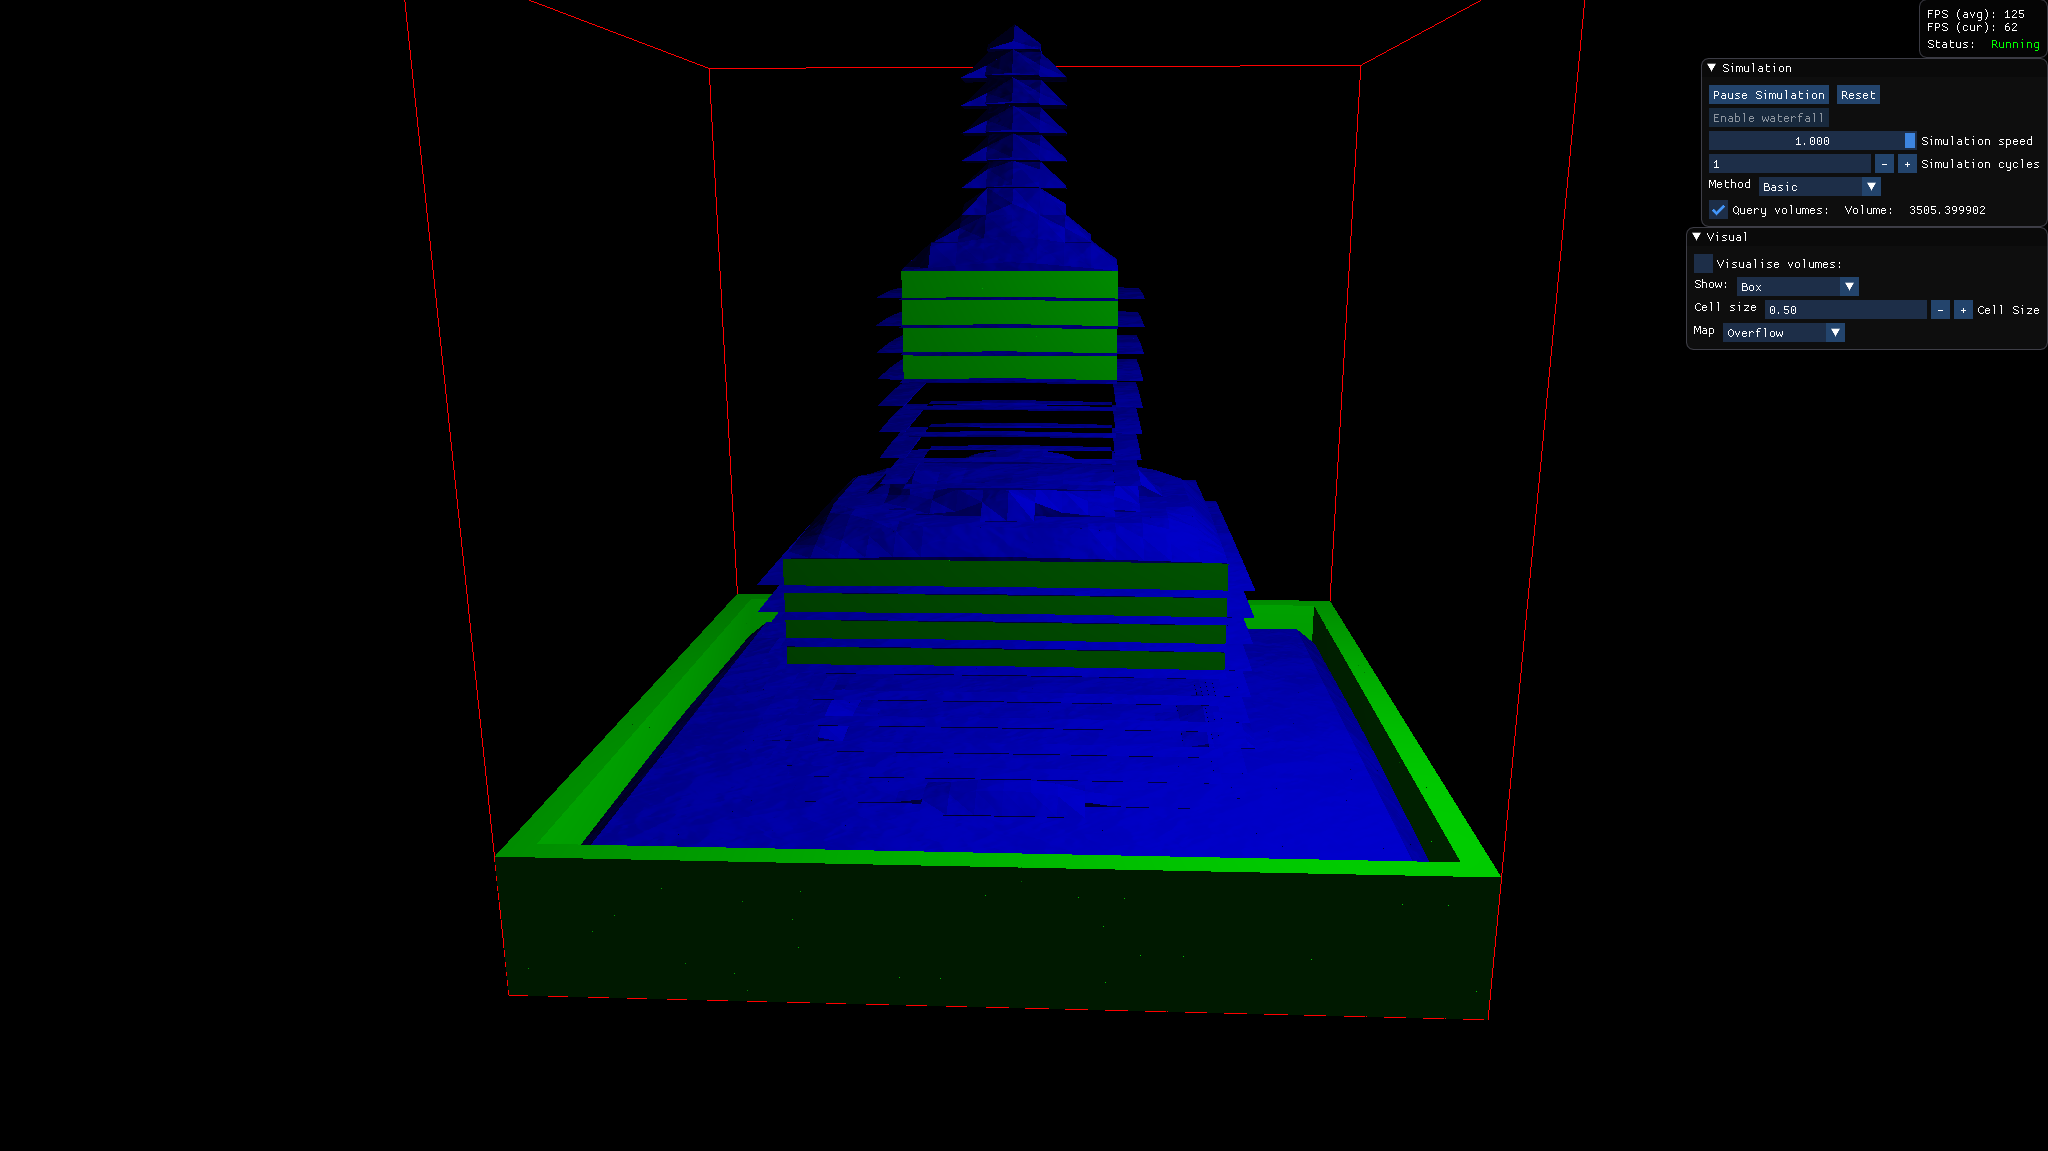
\includegraphics[width=0.5\linewidth]{obrazky-figures/cellular2.png}\hfill
	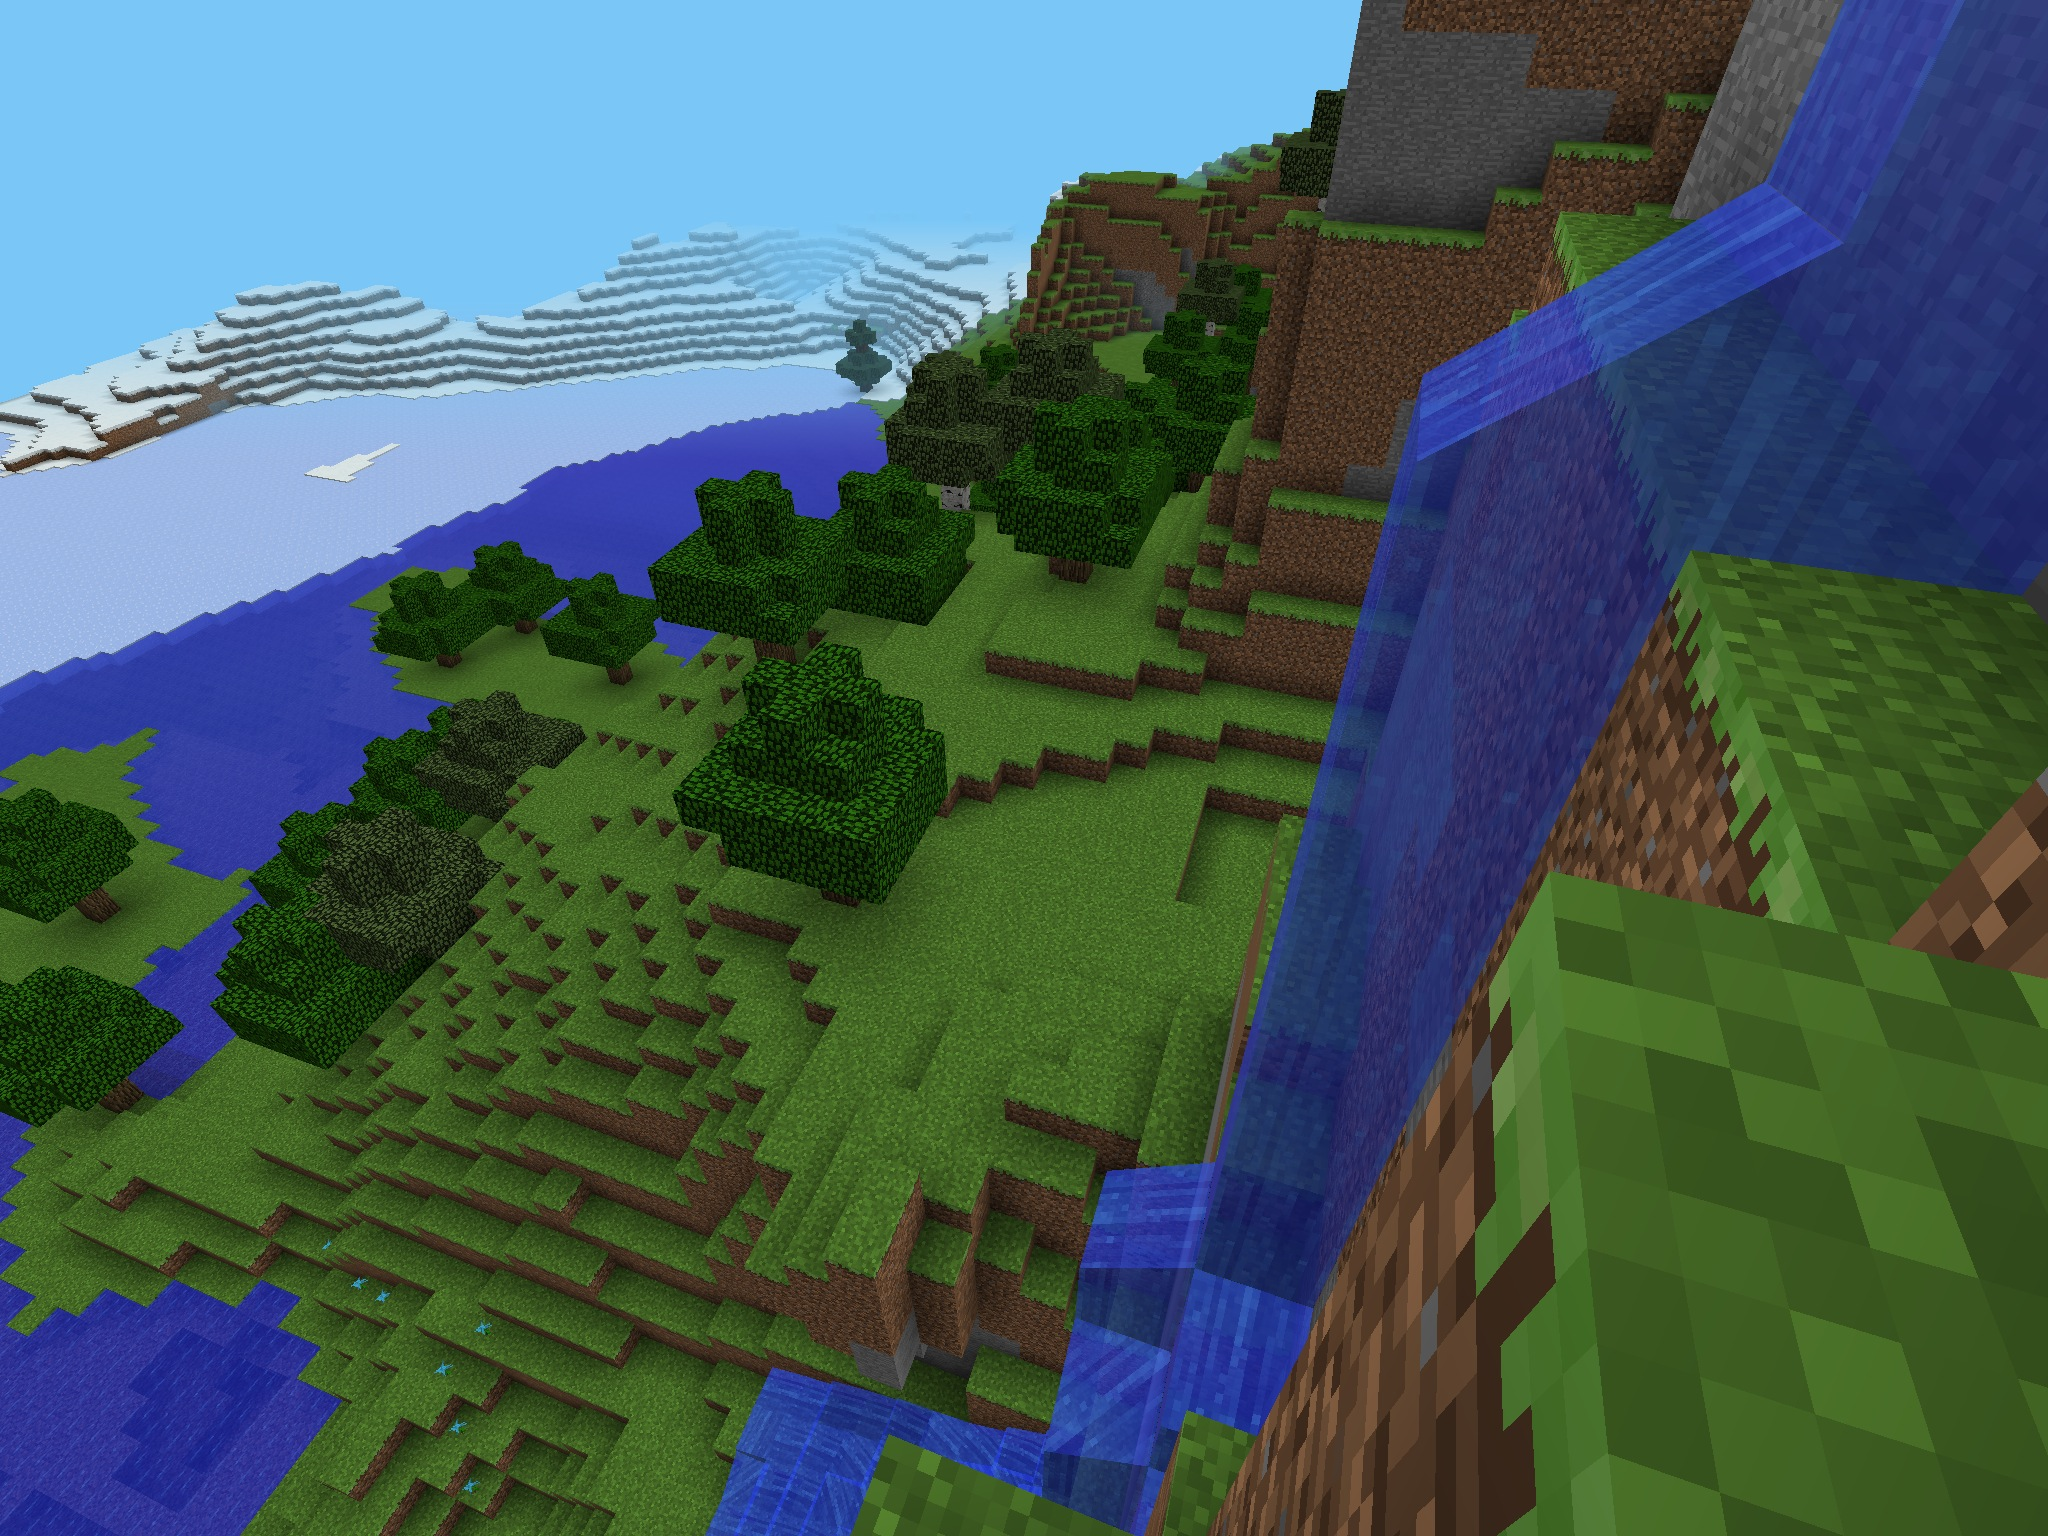
\includegraphics[width=0.5\linewidth]{obrazky-figures/miecraft.jpg}\hfill
	\caption{\textbf{Příklady celulárních simulací.} Na horním obrázku je simulace vytvořená během studia společně s~Bc. Petr Flajšingr. Na spodním obrázku je ukázána simulace vody ve známé hře Minecraft}
	\textbf{Zdroj: } \url{https://github.com/Nirvanios/Water_simulation-cellular_automaton}
	\textbf{Zdroj: } \url{https://mcpedl.com/ayay/}
	\label{fig:SWE}
\end{figure*}

\section{Lagrangeova metoda toku}
Základem Lagrangeovy metody toku není sledování vymezeného prostoru, kde se může kapalina pohybovat, jako je tomu u~Eulerovy metody, ale sledovaní kapaliny samotné. Lagrangeova metoda se tak soustředí na kapalinu samotnou, kterou dělí na samostatné části. Můžeme tedy říci, že se jedná o~částicovou metodu, kde každá taková částice kapaliny nese specifické parametry jako hustotu, tlak, hmotnost a jiné. Pomocí těchto parametrů pak ovlivňuje ostatní částice v~okolí a tím i celou masu kapaliny.

Jak z~popisu vyplývá, tyto metody nejsou v~prostoru omezeny žádnou mřížkou, či jinou strukturou, limitující prostor dané simulace. A~ačkoliv z~nutnosti mít mřížku nevzniká vysoká paměťová náročnost, vyvstává nám paměťová náročnost v~podobě počtu částic. Chceme-li mít dostatečně přesnou a jemnou simulaci, je nutné mít vysoký počet částic. Počty částic se mohou pohybovat v~řádech od desítek tisíc až po jednotky či desítky miliónů. Předpokládáme-li tedy vysoký počet částic a skutečnost, že každá částice o~sobě musí nést mnoho informací jako je rychlost, pozice, hmotnost a další, musíme zároveň počítat s~paměťovými nároky na jiném místě.

\subsection{Smoothed Particle Hydrodynamics}
\label{chapter:SPH}
Smoothed Particle Hydrodynamics (dále jen SPH) je dnes jednou z~nejpoužívanějších metod částicové simulace kapalin. Tato metoda byla představena autory Gingold a Monaghan \cite{Monaghan77} a Lucy \cite{Lucy77}, původně pro řešení problému v~teoretické astrofyzice. Postupem času se z~ní ale stala velice populární metoda, která se dočkala několika rozšíření a modifikací a začala se používat nejen v~astrofyzice, ale také v~balistice, vulkanologii a především obecně v~oblastech simulace tekutin a jiných spojitých mas.

SPH je Lagrangeova metoda, tedy základem jsou tedy částice. Každá částice nese několik konkrétních hodnot, jako je hmotnost, pozice a vektor rychlosti a navíc ještě několik dalších hodnot, vztahujících se k~danému problému, jako je hustota hmotnosti, tlak nebo třeba teplota. Jedná se o~integrační metodu, kde je výpočet atributu $A(\mathbf{r})$ nad prostorem $\Omega$ definován pomocí rovnice \ref{eq:SPHint},
\begin{equation}
	A_I(\mathbf{r}) = \int_\Omega A(\mathbf{r}')W(\mathbf{r} - \mathbf{r'},h)\mathbf{dr}'
	\label{eq:SPHint}
\end{equation}
kde $r$ značí pozici v~prostoru, $W$ je vyhlazovací jádro (smoothing kernel) a $h$ je šířka jádra. Šířka jádra, nazývaná také vyhlazovací poloměr (smoothing radius) pak ovlivňuje kvalitu a stabilitu simulace.
Numerický výpočet je pak zobrazen rovnicí \ref{eq:SPHsum},

\begin{equation}
	A_S(\mathbf{r}) = \sum_j A_j V_j W(\mathbf{r} - \mathbf{r_j},h)
	\label{eq:SPHsum}
\end{equation}

\begin{equation}
	V~= \frac{m}{\rho}
	\label{eq:volume}
\end{equation}
kde je integrál aproximovaný pomocí sumy přes všechny částice $j$ a $V$ je objem v~prostoru, který částice zaujímá a je vypočítaný pomocí známé rovnice \ref{eq:volume}, kde $m$ je hmotnost částice a $\rho$ je hustota hmotnosti částice.  \cite{KelagerSPH}

\subsubsection{Vyhlazovací jádro}
Vyhlazovací jádro je jednou z~nejdůležitějších součástí celého SPH algoritmu a výběr správného jádra má tedy značný vliv na kvalitu a stabilitu simulace. Vhodné jádro musí splňovat dvě důležité podmínky.
\begin{equation}
	\int_\Omega W(\mathbf{r} - \mathbf{r}', h)\mathbf{dr}' = 1
	\label{eq:SPHCond1}
\end{equation}

\begin{equation}
	\lim{h \to 0} W(\mathbf{r} - \mathbf{r}',h) = \delta(\mathbf{r} - \mathbf{r}')
	\label{eq:SPHCond2}
\end{equation}

\begin{equation} \label{eq:dirac}
	\begin{gathered}
		\delta(x) =
		\begin{cases}
			\infty & \quad ||\mathbf{r}|| = 0 \\
			0      & \quad \text{jinak}
		\end{cases}
	\end{gathered}
\end{equation}
První podmínka \ref{eq:SPHCond1} nám udává, že jádro musí být normalizované, a nemůže nám tedy nikterak ovlivnit hodnoty, s~nimiž pracuje. Druhá podmínka \ref{eq:SPHCond2}, kde $\delta$ značí Diracovu delta funkci \ref{eq:dirac}, nám pak limituje počet interpolantů. Značí nám tedy, že výsledek je ovlivněn pouze několika body v~okolí a body příliš vzdálené v~prostoru nám neovlivňují výsledek. V~původním článku autoři pro výpočet použili jedno-dimenzionální Gaussovské jádro. Jako další možnost je použít B-Splajn, kvintický splajn \cite{Liu2010} nebo například polynomiální kernel 6. stupně \cite{Muller03}.

\begin{equation}
	W_{Gauss}(x,h) = \frac{1}{h\sqrt{\pi}}e^{-(x^2/h^2)}
	\label{eq:1DGauss}
\end{equation}

\begin{equation}
	W_{Poly6}(\mathbf{r},h) = \frac{315}{64 \pi h^9}
	\begin{cases}
		(h^2 - ||\mathbf{r}||^2)^3 & \quad 0 \leq ||\mathbf{r}|| \leq h \\
		0                          & \quad \text{jinak}
	\end{cases}
	\label{eq:kernelPoly6}
\end{equation}

\begin{figure}[hbt]
	\centering
	\captionsetup{justification=centering}
	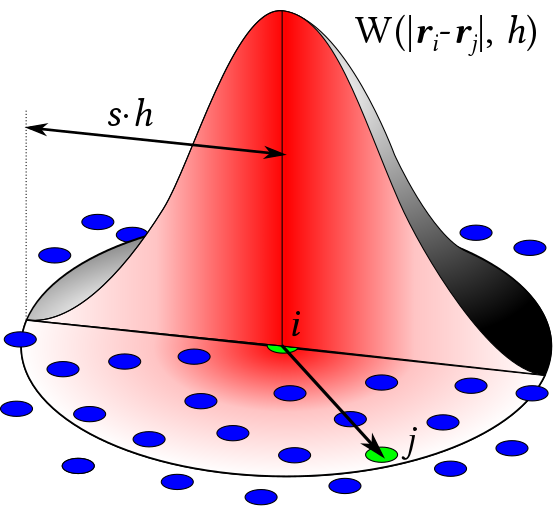
\includegraphics[width=0.4\textwidth]{obrazky-figures/SPHInterpolationColorsVerbose.png}
	\caption{\textbf{Vyhlazovací jádro.} Vizualizace vyhlazovacího jádra. Zelené body $i$, $j$ jsou právě počítané částice, kde počítáme určitou veličinu pro částici $i$. $h$ nám pak udává poloměr jádra, se kterým pracuje.}
	\textbf{Zdroj: } \url{https://en.wikipedia.org/wiki/Smoothed-particle_hydrodynamics}
	\label{fig:Kernel}
\end{figure}

\subsubsection{Hustota hmotnosti}
První veličinou, kterou je nutné vypočítat, je hustota hmotnosti pro každou konkrétní částici. Algoritmus SPH předpokládá, že hmotnost všech částic je během algoritmu neměnná a zároveň dopředu známá hodnota. Využijeme-li tedy rovnice \ref{eq:SPHsum} a dosadíme rovnici \ref{eq:volume}, vznikne nám následující rovnice pro výpočet hustoty.


\begin{equation}
	\begin{split}
		\rho_i  & = \sum_i \rho_j V_j W(\mathbf{r_i} - \mathbf{r_j},h) \\
		& = \sum_i m_j W(\mathbf{r_i} - \mathbf{r_j},h)
	\end{split}
	\label{eq:MassDensity}
\end{equation}

\subsubsection{Tlak}
Tlak a síly působící díky tlaku jsou nesmírně důležité z~důvodu zachování nestlačitelnosti kapaliny. Dostane-li se větší shluk částic do jednoho místa, dojde k~lokálnímu zvýšení hustoty a tedy i tlaku a v~důsledku toho je nutné aplikovat takové síly, aby se shluk rozprostřel na větším prostoru. Tato síla je pak v~Navier-Stokesových rovnicích \ref{eq:NavierStokes} reprezentována termem $-\nabla p$. Chceme-li pak vypočítat tlakovou sílu působící na částici, můžeme opět aplikovat rovnici \ref{eq:SPHsum}, na ni rovnici \ref{eq:volume} a dosadit právě zmíněný term z~Navier-Stokesových rovnic.

\begin{equation}
	f^{tlak}_i = -\nabla p_i  & = \sum_i p_j \frac{m_j}{\rho_j} \nabla W(\mathbf{r_i} - \mathbf{r_j},h)
\end{equation}

Taková rovnice by však neprodukovala správné výsledky. Uvažujeme-li simulaci se dvěma částicemi, přijdeme na jeden zásadní problém, a to, že pomocí této rovnice bychom neobdrželi symetrické síly. Každá částice má lehce odlišný tlak, a proto tedy budou působící síly asymetrické. Existuje více způsobů jak symetrizovat tyto síly v~kontextu SPH. Nejjednodušším příkladem je následující rovnice. \cite{KelagerSPH} \cite{Monaghan92}

\begin{equation}
	f^{tlak}_i = -\sum_{i} \frac{p_i + p_j}{2} \frac{m_j}{\rho_j} \nabla W(\mathbf{r_i} - \mathbf{r_j},h)
	\label{eq:PressForce}
\end{equation}

Nyní, když máme symetrickou tlakovou sílu, je poslední neznámou hodnota parametru $p$, označujícího tlak v~místě částice. Tuto hodnotu tlaku lze obdržet ze stavové rovnice ideálního plynu,
\begin{equation}
	p = k\rho
	\label{eq:idealGas}
\end{equation}
kde $p$ je hledaný tlak, $k$ je plynová konstanta závislá na teplotě a $\rho$ je hustota vypočítaná pomocí rovnice \ref{eq:MassDensity}. Pro dosažení lepších výsledků lze také využít následující rovnice,

\begin{equation}
	p_i = k(\rho_i - \rho_0)
	\label{eq:idealGasRest}
\end{equation}
kde $\rho_0$ označuje klidovou hustotu kapaliny. Jelikož síla závisí na gradientu pole tlaku, tento posun neovlivní výsledek sil, nicméně může učinit simulaci o~něco stabilnější.

Posledním problémem je výše popsané vyhlazovací jádro \ref{eq:kernelPoly6}. Zmíněné jádro má totiž snižovat velikosti odpuzujících sil, čím blíže částice jsou. Nastane-li tedy vysoký shluk částic, jádro není schopné produkovat dostatečné síly pro rovnoměrné rozprostření částic. Proto bylo navrženo \cite{Desbrun96} lepší jádro, schopné dané částice od sebe odtrhnout.

\begin{equation}
	W = (\mathbf{r}, h) = \frac{15}{\pi h^6}
	\begin{cases}
		(h - \mathbf{r})^3 & \quad 0 \leq ||\mathbf{r}|| \leq h \\
		0                  & \quad \text{jinak}
	\end{cases}
	\label{eq:pressureKernel}
\end{equation}

\subsubsection{Viskozita}
Pokud bychom vzali dosavadní rovnice, aplikovali je a postoupili k~integraci (viz. níže), dostali bychom simulaci neviskózní kapaliny. V~reálném světě má však za běžných podmínek každá kapalina určitou viskozitu. Viskozitu můžeme chápat jako působení sil bránící kapalině ve změně tvaru z~důvodu vnitřního tření. Pro zavedení rovnice na výpočet síly působící díky viskozitě použijeme opět Navier-Stokesovy rovnice, tentokrát term pro viskozitu $\mu \nabla^2\mathbf{u}(\mathbf{r_i})$ a opět obecnou rovnici pro SPH \ref{eq:SPHsum} a rovnici pro objem \ref{eq:volume}.

\begin{equation}
	f^{viskozita}_i = \mu \nabla^2\mathbf{u}(\mathbf{r_i}) = \mu \sum_i \mathbf{u_j} \frac{m_j}{\rho_j} \nabla^2 W(\mathbf{r_i} - \mathbf{r_j},h)
\end{equation}

Zde nastává stejný problém, jako u~tlakových sil, a to že jsou síly opět asymetrické. Správného výsledku pak můžeme dosáhnout následující rovnicí. \cite{Muller03}

\begin{equation}
	f^{viskozita}_i = \mu \sum_i m_j \frac{\mathbf{u_i} - \mathbf{u_j}}{\rho_j} \nabla^2 W(\mathbf{r_i} - \mathbf{r_j},h)
	\label{eq:ViscForce}
\end{equation}

Viskozita je vlastnost tekutiny, která do celého systému ze svého principu nepřináší energii, a tedy v~celé tekutině nikterak nevzrůstá rychlost. Avšak jak polynomiální jádro šestého řádu \ref{eq:kernelPoly6}, tak jádro použité pro výpočet tlaku \ref{eq:pressureKernel}, může do systému takové zvýšení energie zanést. Hledáme tedy takové jádro, které nám pouze snižuje velikost sil v~závislosti na velikosti viskozity. Následující jádro takovou podmínku splňuje. \cite{Muller03}

\begin{equation}
	W = (\mathbf{r}, h) = \frac{15}{2 \pi h^3}
	\begin{cases}
		-\frac{||\mathbf{r}||^3}{2h^3} + \frac{||\mathbf{r}||^2}{h^2} + \frac{h}{2||\mathbf{r}||} & \quad 0 \leq ||\mathbf{r}|| \leq h \\
		0                                                                                         & \quad \text{jinak}
	\end{cases}
	\label{eq:pressureKernel}
\end{equation}

\begin{figure}[hbt]
	\centering
	\captionsetup{justification=centering}
	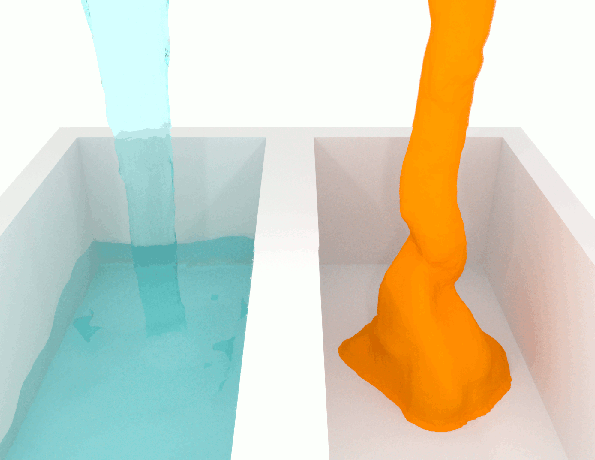
\includegraphics[width=0.5\textwidth]{obrazky-figures/viskozita.PNG}
	\caption{\textbf{Viskozita.} Případy různé viskozity, kapalina vpravo se mnohem více brání toku než kapalina vlevo.}
	\textbf{Zdroj: } \url{https://en.wikipedia.org/wiki/Fluid_animation}
	\label{fig:Vics}
\end{figure}

\subsubsection{Povrchové napětí}
Povrchové napětí je síla působící na vnější povrch kapaliny, přesněji řečeno se jedná o~nerovnováhu sil. Každá molekula kapaliny vytváří síly přitahující ostatní molekuly v~kapalině, jež jsou poblíž. Uvnitř kapaliny jsou síly vyrovnané, ale jak znázorňuje obr. \ref{fig:SurTen}, molekuly na okraji kapaliny jsou pouze přitahovány do pomyslného středu kapaliny. Povrchové napětí sice není přítomno v~Navier-Stokesových rovnicích, nicméně se jedná o~velice důležitou součást chování kapalin. Povrchové napětí totiž zapříčiňuje minimalizaci povrchu kapaliny, kterou můžeme v~přírodě pozorovat. \cite{KelagerSPH}

\begin{equation}
	f_i^{povrchové napětí} = \sigma \nabla^2 c_i \frac{\mathbf{n}_i}{||\mathbf{n}_i||}
	\label{eq:SurfTen}
\end{equation}

\begin{figure}[hbt]
	\centering
	\captionsetup{justification=centering}
	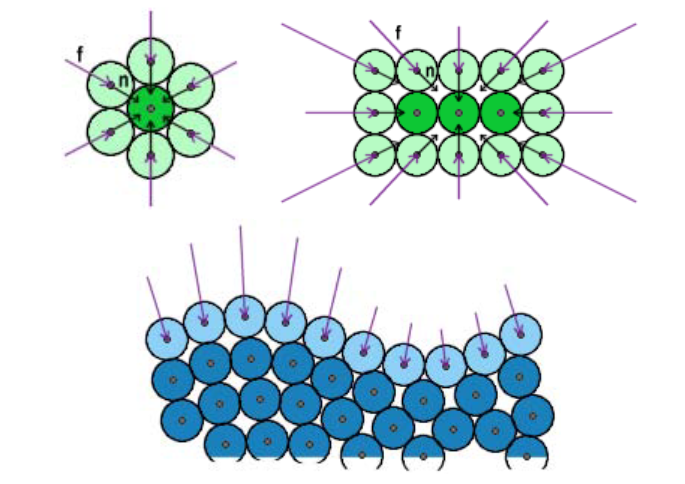
\includegraphics[width=0.7\textwidth]{obrazky-figures/SurfTens.png}
	\caption{\textbf{Povrchové napětí.} Různé případy povrchového napětí}
	\textbf{Zdroj: } Lagrangian Fluid Dynamics Using Smoothed Particle Hydrodynamics \cite{KelagerSPH}
	\label{fig:SurTen}
\end{figure}

Pomocí výše zmíněné rovnice pak lze vypočítat sílu povrchového napětí. V~rovnici $\sigma$ představuje koeficient povrchového napětí, specifický pro danou kapalinu, $c$ je tzv. barevné pole a $\mathbf{n}$ je normála povrchu kapaliny směřující dovnitř. Barevné pole $c$ je definováno následovně.

\begin{equation}
	c_i =
	\begin{cases}
		1 & \quad  \text{na pozici částice } i \\
		0 & \quad  \text{jinde}
	\end{cases}
\end{equation}

S~pomocí rovnice \ref{eq:SPHsum} lze pak pole $c_i$ vypočítat následovně.

\begin{equation}
	\begin{split}
		c_i =   & \sum_j c_j V_j \nabla^2 W(\mathbf{r_i} - \mathbf{r_j},h) \\
		=   & \sum_j V_j \nabla^2 W(\mathbf{r_i} - \mathbf{r_j},h)
	\end{split}
	\label{eq:ColorField}
\end{equation}

Z~gradientu barevného pole pak lze získat normálu povrchu $\mathbf{n}_i$.
\begin{equation}
	\mathbf{n}_i = \nabla c_i
	\label{eq:SurfNormal}
\end{equation}

Podmínka vyhodnocení je omezena členem $\frac{\mathbf{n}_i}{||\mathbf{n}_i||}$, kde $||\mathbf{n}_i||$ nabývá nenulových hodnot pouze blízko okraje kapaliny. Pokud je však $||\mathbf{n}_i||$ příliš malé, způsobuje numerickou nestabilitu řešení, a proto se síla povrchového napětí počítá jen v~případě, kdy $||\mathbf{n}_i||$ překročí jistý práh.


\subsubsection{Síly}
Síly působící na kapalinu můžeme rozdělit do dvou kategorií, vnitřní a vnější síly. Pro výpočet celkové síly působící na jednu částici v~systému pak stačí vnější a vnitřní síly sečíst. Vnitřní a vnější síly jsou definovány následovně, \cite{KelagerSPH}

\begin{equation}
	f^{vnitřní} = f^{tlak} + f^{viskozita}
	\label{eq:ForceInt}
\end{equation}

\begin{equation}
	f^{vnější} = f^{\text{povrchové napětí}} + f^{gravitace}
	\label{eq:ForceExt}
\end{equation}
kde je síla působící z~důvodu gravitace vyjádřena následovně, přičemž $g$ značí gravitační zrychlení.

\begin{equation}
	f^{gravitace} = \rho g
\end{equation}

Posledním důležitým krokem je výpočet zrychlení částice z~důvodu působení sil.

\begin{equation}
	a_i = \frac{f^{vnejsi} + f^{vnitri}}{\rho}
	\label{eq:Acc}
\end{equation}

\subsubsection{Integrace}
Nyní máme vše potřebné pro základní SPH simulaci, nicméně pouhým výpočtem výše popsaných vlastností hodnot nedostaneme tekoucí kapalinu. Je nutné každou částici vždy posunout v~čase a prostoru na základě předchozí pozice, rychlosti a působících sil. Existuje několik přístupů jak numericky řešit posun částic v~čase a prostoru.

Mezi nejznámější a nejjednodušší metodu numerické integrace patří Eulerova metoda. V~její nejjednodušší formě se pozice i rychlost aktualizují zároveň na základě vypočtených hodnot.

\begin{equation}
	\mathbf{u}_{t + \Delta t} = \mathbf{u}_t + \Delta t \mathbf{a}_t
\end{equation}

\begin{equation}
	\mathbf{r}_{t + \Delta t} = \mathbf{r}_t + \Delta t \mathbf{u}_t
\end{equation}

Existuje lehké zlepšení metody, ve kterém se následující pozice počítá z~již vypočítané rychlosti. Výpočet pozice tedy závisí na výpočtu rychlosti. \cite{KelagerSPH}

\begin{equation}
	\mathbf{r}_{t + \Delta t} = \mathbf{r}_t + \Delta t \mathbf{u}_{t + \Delta t}
\end{equation}

Dalším vylepšením může být integrační metoda Leap-Frog. Tato metoda vychází z~Eulerovy metody, nicméně zavádí posunutí výpočtu rychlosti v~čase. Výpočet rychlosti je posunut o~$\frac{\Delta t}{2}$, čímž dochází ke \enquote{střídání} výpočtu rychlosti a pozice, viz. obr. \ref{fig:LeapFrog}.

\begin{equation}
	\mathbf{u}_{t + \frac{\Delta t}{2}} = \mathbf{u}_{t - \frac{\Delta t}{2}} t \mathbf{a}_t
	\label{eq:LeapVel}
\end{equation}

\begin{equation}
	\mathbf{r}_{t + \Delta t} = \mathbf{r}_t + \Delta t \mathbf{u}_{t + \frac{\Delta t}{2}}
	\label{eq:LeapPos}
\end{equation}

\begin{figure}[hbt]
	\centering
	\captionsetup{justification=centering}
	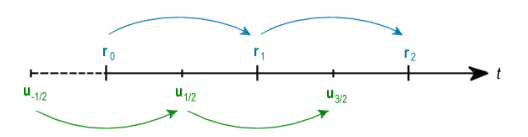
\includegraphics[width=0.7\textwidth]{obrazky-figures/leapFrog.PNG}
	\caption{\textbf{Leap-Frog integrace.} Vyobrazení posunutí integrace rychlosti a pozice mezi sebou.}
	\textbf{Zdroj: } Lagrangian Fluid Dynamics Using Smoothed Particle Hydrodynamics \cite{KelagerSPH}
	\label{fig:LeapFrog}
\end{figure}

\subsubsection{Algoritmus simulace}

\begin{center}
	\begin{czechalgorithm}[H] \label{alg:SPH}
		inicializace částice v~prostoru a potřebných konstant\\
		\While {True}{
			\ForEach{\text{particle}} {\\
				vypočti hustotu (viz. \ref{eq:MassDensity})\\
				vypočti tlak (viz. \ref{eq:idealGasRest})\\
			}\\
			\\
			\ForEach{\text{particle}} {\\
				vypočti tlakovou sílu $f^{tlak}_i$ (viz. \ref{eq:PressForce})\\
				vypočti viskózní sílu $f^{viskozita}_i$ (viz. \ref{eq:ViscForce})\\
				vypočti vlastní hodnotu barevného pole $c_i$ (viz. \ref{eq:ColorField})\\
				vypočti normálu povrchu kapaliny $\mathbf{n}_i$ (viz. \ref{eq:SurfNormal})\\
				vypočti sílu povrchového napětí $f^{\text{povrchové napětí}}_i$ (viz. \ref{eq:SurfTen})\\
				$f^{vnitrni} = f^{tlak}_i f^{viskozita}_i$ \\
				$f^{vnitrni} = f^{\text{povrchové napětí}}_i + f^{gravitace}_i$\\
				$f = f^{vnejsi} + f^{vnitrni}$ (viz. \ref{eq:ForceExt} a \ref{eq:ForceInt})\\
				vypočti zrychlení $a_i$ (viz. \ref{eq:Acc})\\
				integruj a posuň částici v~čase (viz. \ref{eq:LeapPos} a (viz. \ref{eq:LeapPos})\\
			}\\
		}
		\caption{SPH Simulace}
	\end{czechalgorithm}
\end{center}

\begin{figure*}[h]\centering
	\centering
	\captionsetup{justification=centering}
	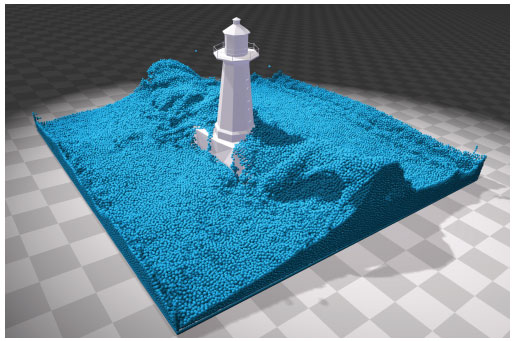
\includegraphics[width=0.5\linewidth]{obrazky-figures/SPHSim1_01.jpg}\hfill
	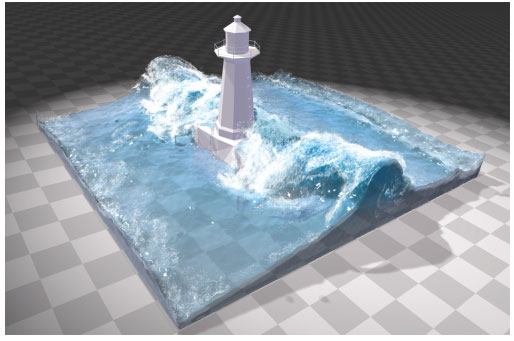
\includegraphics[width=0.5\linewidth]{obrazky-figures/SPHSim1_02.jpg}\hfill
	\caption{\textbf{Příklady SPH Simulace.} Na levém obrázku je simulace zobrazená pomocí jednotlivých částic. Na pravém obrázku je ukázána vyrenderovaná hladina}
	\textbf{Zdroj: } SPH Fluids in Computer Graphics \cite{Ihmsen14}
	\label{fig:SPHFigure}
\end{figure*}

\chapter{Návrh řešení}
\label{chapter:navrh_resení}
Tato práce si klade za cíl implementovat práci \cite{Evap&Cond} autorů Hochstetter a Kolb z~University of Siegen v~Německu. Ačkoliv se s~kondenzací a vypařováním setkáváme běžně každý den, v~rámci simulace kapalin a počítačové grafiky není mnoho prací věnujících se tomuto tématu. Z~tohoto důvodu se pomocí zmíněného článku snaží autoři představit novou metodu, jak takové změny skupenství simulovat. Autoři se rozhodli využít dvou metod simulace, pro kapalné skupenství využili metodu Smoothed Particle Hydrodynamics (viz. kapitola \ref{chapter:SPH}), plynné skupenství pak bylo simulováno za využití mřížkové metody (viz. kapitola \ref{chapter:Grid}). Pro kondenzaci na povrchu pevných těles následně využili textur nesoucích potřebné údaje. Níže je celá metoda vypařování a kondenzace podrobněji popsána, celý popis pak vychází z~článku napsaného autory. \cite{Evap&Cond}

\subsubsection{Základní princip}
Popisovaná simulace se skládá ze tří částí, částicový systém pro simulaci kapalného stavu, mřížkový systém pro simulaci plynného stavu a textury udržující informace o~množství kondenzace na pevných tělesech. Principy SPH simulace a mřížkové metody již byly popsány výše v~kapitolách \ref{chapter:SPH} a \ref{chapter:Grid} respektive, nicméně pro správné fungování cyklu vypařování a kondenzace je nutné do obou systémů zavést novou veličinu, a to teplotu.

Pro mřížkovou metodu se jedná o~pouhé advekování teploty a hustoty pomocí pole vektorů rychlostí. Postup veličin je popsán následujícími rovnicemi.
\begin{equation}
	\frac{\partial T}{\partial t} = -(\mathbf{u} \cdot \nabla)T
\end{equation}

\begin{equation}
	\frac{\partial \rho}{\partial t} = -(\mathbf{u} \cdot \nabla)\rho
\end{equation}

Abychom zachovali vlastnost plynů, že horký plyn stoupá a hustý plyn klesá, je nutné zavést do systému vztlakovou sílu. Ta je popsána následující rovnicí,

\begin{equation}
	f_{buoy} = -\alpha \rho \hat{\mathbf{g}} + \beta(T - T_{amb})\hat{\mathbf{g}}
\end{equation}
kde $\alpha$ a $\beta$ jsou předem definované konstanty a $\hat{\mathbf{g}}$ je normalizovaný vektor gravitačního zrychlení.

Pro SPH simulaci je nutné počítat pro každou částici také teplotu. Pro modelování teploty v~rámci kapaliny využili autoři článku rovnici vytvořenou dvojící Cleary a Monaghan \cite{Cleary99}.

\begin{equation}
	\frac{\partial T}{\partial t} = \frac{V_1}{m_i C_i} \sum_j \frac{4 k_i k_j}{k_i + k_j} V_j \frac{(T_i - T_j)}{||\mathbf{r}_i - \mathbf{r}_j||}\nabla W(\mathbf{r} - \mathbf{r_j},h)
\end{equation}

Nakonec jsou vytvořeny textury pro pevné tělesa. Každému tělesu náleží několik textur. Základní textura v~každém texelu obsahuje množství zkondenzované kapaliny. Použitím textury a texelů menší než je částice z~SPH simulace je docíleno jemnějšího detailu při kondenzaci. Dále máme přepočítanou texturu obsahující maximální množství kapaliny v~daném texelu a texturu obsahující mapu pozic pro vytváření SPH částic. Další textury obsahují například teplotu, případně historii kondenzace.

\subsubsection{Míra kondenzace a vypařování}
Při vypařování a kondenzaci je nutné zjistit množství hmoty, které se transformuje z~jednoho skupenství do druhého, pro výpočet změny hmotnosti v~povrchu kapaliny je nabízen následující vzorec založený na empirických datech. \cite{SMITH94}

\begin{equation}
	\frac{\partial m_s}{\partial t} = A_s(a + b \cdot ||\mathbf{u}||)(p_s^{sat} - p_c)
	\label{eq:EvapRate}
\end{equation}

Kde $A_s$ je plocha kontaktu kapaliny, $a$ a $b$ jsou konstanty ovlivňující vypařování a $p_s^{sat}$ je tlak nasycených výparů u~povrchu kapaliny a $p_c$ je tlak výparu v~buňce. Hodnoty tlaků jsou vypočítány následujícími rovnicemi. \cite{yau1996short}

\begin{equation}
	p_c = \frac{m_c R_w(T_c - 273.15^{\circ}C)}{V_c}
\end{equation}

\begin{equation}
	p_s^{sat} = 611.2\text{Pa} * e^{\frac{17,62 \cdot T_s}{243.12^{\circ}C + T_s}}
\end{equation}

Rovnice \ref{eq:EvapRate} nám tedy říká míru vypařování z~povrchu kapaliny, nicméně míru kondenzace můžeme vyjádřit s~pomocí stejné rovnice. V~závislosti na znaménku výsledku dané rovnice pak určíme, zda se jedná o~kondenzaci či vypařování. Dostáváme tedy následující rovnice,

\begin{equation}
	\text{míraVypařování}(c,s) = \max(\frac{\partial m_s}{\partial t}, 0)
	\label{eq:EvapTrans}
\end{equation}

\begin{equation}
	\text{míraKondenzace}(c,s) = \min(\frac{\partial m_s}{\partial t}, 0), \text{kde } b = 0
	\label{eq:CondTrans}
\end{equation}

přičemž $c$ značí buňku a $s$ značí surfel, tedy povrchovou jednotku kapaliny. Pro zjištění hodnot buňky na konkrétní pozici $\mathbf{r}$ využijeme trilineární interpolace hodnot buněk v~okolí. Rovnice \ref{eq:EvapRate} přináší určitou závislost vypařování na proudění vzduchu v~okolí, nicméně kondenzace v~žádném případě nezávisí na okolní rychlosti vzduchu, proto jej z~rovnice vyškrtneme za pomocí argumentu $b$. Nakonec musíme při každém přenosu zajistit, aby se z~kapaliny odebralo stejné množství hmotnosti, jako je přijato do plynné fáze. Snažíme se tedy zajistit zákon o~zachování hmotnosti a nezpůsobovat úbytek či přírůstek hmotnosti v~celém systému simulace.

\subsubsection{Simulace}
Pro správné fungování simulace, přenosů tepla a hmotností je nutné veškeré systémy propojit. Je zapotřebí přenos teplot mezi kapalinou a výpary a texturami a částicemi. Pevná tělesa jsou reprezentována pomocí částic, a to z~důvodu snadnější interakce kapalina~$\leftrightarrow$~\mbox{těleso} nejen v~rámci sil, ale i přenosu tepla. Zároveň musí docházet k~přenosu hmotnosti mezi všemi třemi systémy. Celé propojení je znázorněné na obrázku \ref{fig:EvapCycle}.

\begin{figure}[hbt]
	\centering
	\captionsetup{justification=centering}
	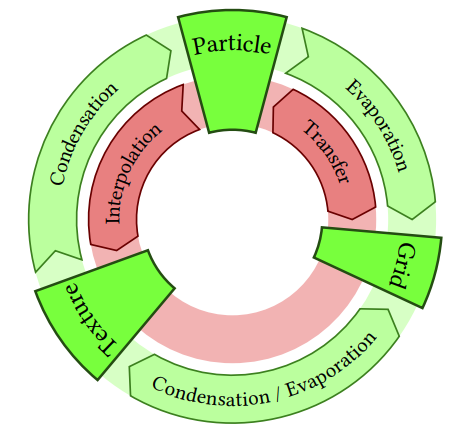
\includegraphics[width=0.4\textwidth]{obrazky-figures/evapCycle.PNG}
	\caption{\textbf{Propojení tří systémů.} Zelený kruh zobrazuje přenos hmotnosti a červený kruh přenos teploty.}
	\textbf{Zdroj: } Evaporation and condensation of SPH-based fluids \cite{Evap&Cond}
	\label{fig:EvapCycle}
\end{figure}

\subsubsection{Přenos tepla}
Pro fungování simulace je nutné vytvořit přenos tepla částice $\leftrightarrow$ buňka a jelikož se pevná tělesa sestávají z~částic tak také částice $\leftrightarrow$ texel.

Představíme-li si celý systém kapaliny a jejích výparů, je zřejmé, že z~jedné buňky obsahující výpary může dojít k~přenosu tepla do několika částic zároveň, a naopak z~jedné částice může dojít k~přenosu tepla do více buněk. Autoři článku tedy představují dvě rovnice, rovnici \ref{eq:Part2Cell} pro přenos částice $\rightarrow$ buňka a rovnici \ref{eq:Cell2Part} pro přenos buňka $\rightarrow$ částice.

\begin{equation}
	\frac{\partial T_i}{\partial t} = \frac{1}{\rho_i C_i} A_i \sum_c \frac{4 k_i k_c}{k_i + k_c}(T_i - T_c)a_{ic}
	\label{eq:Part2Cell}
\end{equation}

\begin{equation}
	\frac{\partial T_c}{\partial t} = \frac{1}{\rho_c C_c} A_i \sum_j a_{jc}\frac{4 k_j k_c}{k_j + k_c}(T_c - T_j)A_j
	\label{eq:Cell2Part}
\end{equation}

Přenos tepla do textury je pak proveden pouhou interpolací hodnot z~částic pevného tělesa do jednotlivých texelů. Tímto jednoduchým způsobem dostane každý texel vlastní teplotu, nicméně není nutné aplikovat složité vzorce na výpočet a zvyšovat tím tak výpočetní náročnost.

\subsubsection{Přenos hmotnosti}
Přenos mezi texturou a částicemi probíhá pouze jedním směrem, a to texel $\rightarrow$ částice pomocí kondenzace. Pokud se nachází na textuře v~okolí pozic pro generování částic dostatečná hmotnost kondenzované kapaliny, dochází ke generování částice. Dané množství kapaliny je odebráno z~textury a je vytvořena částice o~stejném množství kapaliny.

Výměna hmotnosti mezi texely a buňkami s~výpary je poměrně jednoduchá. Základem je výpočet míry vypařování a kondenzace pomocí vzorců \ref{eq:EvapTrans} a \ref{eq:CondTrans}. Pokud bychom však slepě aplikovali tyto vzorce, mohlo by dojít k~odebrání většího množství hmotnosti kapaliny než je přítomné v~buňce či texelu, případně přesaturování, kdy by bylo obsaženo více než je povolené množství. Z~tohoto důvodu musí být všechny přenosy škálovány podle množství již přítomné kapaliny či výparů.

Pro vypařování a kondenzaci mezi částicemi kapaliny a buňkami platí stejný postup jako mezi texely a buňkami. Musíme dodržet stejná pravidla, nicméně u~částic nedochází ke změně hmotnosti, nýbrž se mění jejich škálovací faktor. Tento faktor pak ovlivňuje veškeré vlastnosti částice, jako je tlak, hustota apod. až na hmotnost, která jím není ovlivněna. V~celé simulaci se snažíme dodržet, aby každá částice měla stejný faktor $w_i = 1$, proto pokud nalezneme částice s~nízkými faktory, můžeme dané částice sloučit a vytvořit jednu s~vyšším faktorem.




\chapter{Implementace}
\label{chapter:implementace}
\section{Použité knihovny}
Pro implementaci byl zvolen jazyk \texttt{c++} ve standardu 20. Pro zjednodušení a automatizaci překladu pak bylo využito nástrojů \texttt{CMake} \footnote{\url{https://cmake.org/}} a \texttt{Ninja} \footnote{\url{https://ninja-build.org/}}. Samotné psaní kódu pak probíhalo ve vývojovém prostředí \texttt{CLion} \footnote{\url{https://www.jetbrains.com/clion/}}, přičemž tvorba shaderů probíhala v~programu \texttt{Visual Studio Code} \footnote{\url{https://code.visualstudio.com/}} s~pomocí pluginu \texttt{GLSL Lint} \footnote{\url{https://marketplace.visualstudio.com/items?itemName=CADENAS.vscode-glsllint}}. Pro správu většiny knihoven třetích stran bylo využito nástrojů \texttt{Hunter} \footnote{\url{https://hunter.readthedocs.io/}} a \texttt{CPM.cmake} \footnote{\url{https://github.com/TheLartians/CPM.cmake}}.
\begin{multicols}{2}
	\begin{itemize}
		\item glm \footnote{\url{https://glm.g-truc.net/}}
		\item GLFW \footnote{\url{https://glfw.org/}}
		\item {fmt} \footnote{\url{https://github.com/fmtlib/fmt}}
		\item spdlog \footnote{\url{https://github.com/gabime/spdlog}}
		\item stb \footnote{\url{https://github.com/nothings/stb}}
		\item libshaderc \footnote{\url{https://github.com/google/shaderc/tree/main/libshaderc}}
		\item toml11 \footnote{\url{https://github.com/ToruNiina/toml11}}
		\item range-v3 \footnote{\url{https://github.com/ericniebler/range-v3}}
		\item tinyobjloader \footnote{\url{https://github.com/tinyobjloader/tinyobjloader}}
		\item camera \footnote{\url{https://learnopengl.com/Getting-started/Camera}}
		\item ffmpeg \footnote{\url{https://ffmpeg.org/}}
	\end{itemize}
\end{multicols}
\chapter{Testování}
\label{chapter:testovani}

\chapter{Závěr}
\label{chapter:zaver}





%===============================================================================
